% 2.	Bouldering:
% •	For each boulder problem, climbers usually have 4 minutes to attempt it. In some competitions, the “4+ rule” applies, allowing climbers to finish their final attempt if they start it before the 4-minute timer expires

\begin{frame}
    \begin{minipage}{0.48\linewidth}
        \textbf{Project Presentation}

        \vspace{0.5em}

        \centering
        \includegraphics[width=\textwidth]{assets/visuals/temporal-action-segmentation-visual.png}
        \cite{ding2023temporal}

        \vspace{0.5em}

        \begin{itemize}
            \item Part of a bigger research project.
            \item Analyze professional climbers behaviors.
        \end{itemize}
    \end{minipage}
    \hfill
    \begin{minipage}{0.48\linewidth}
        \centering
        % TODO: image ou deux des videos du dataset.
        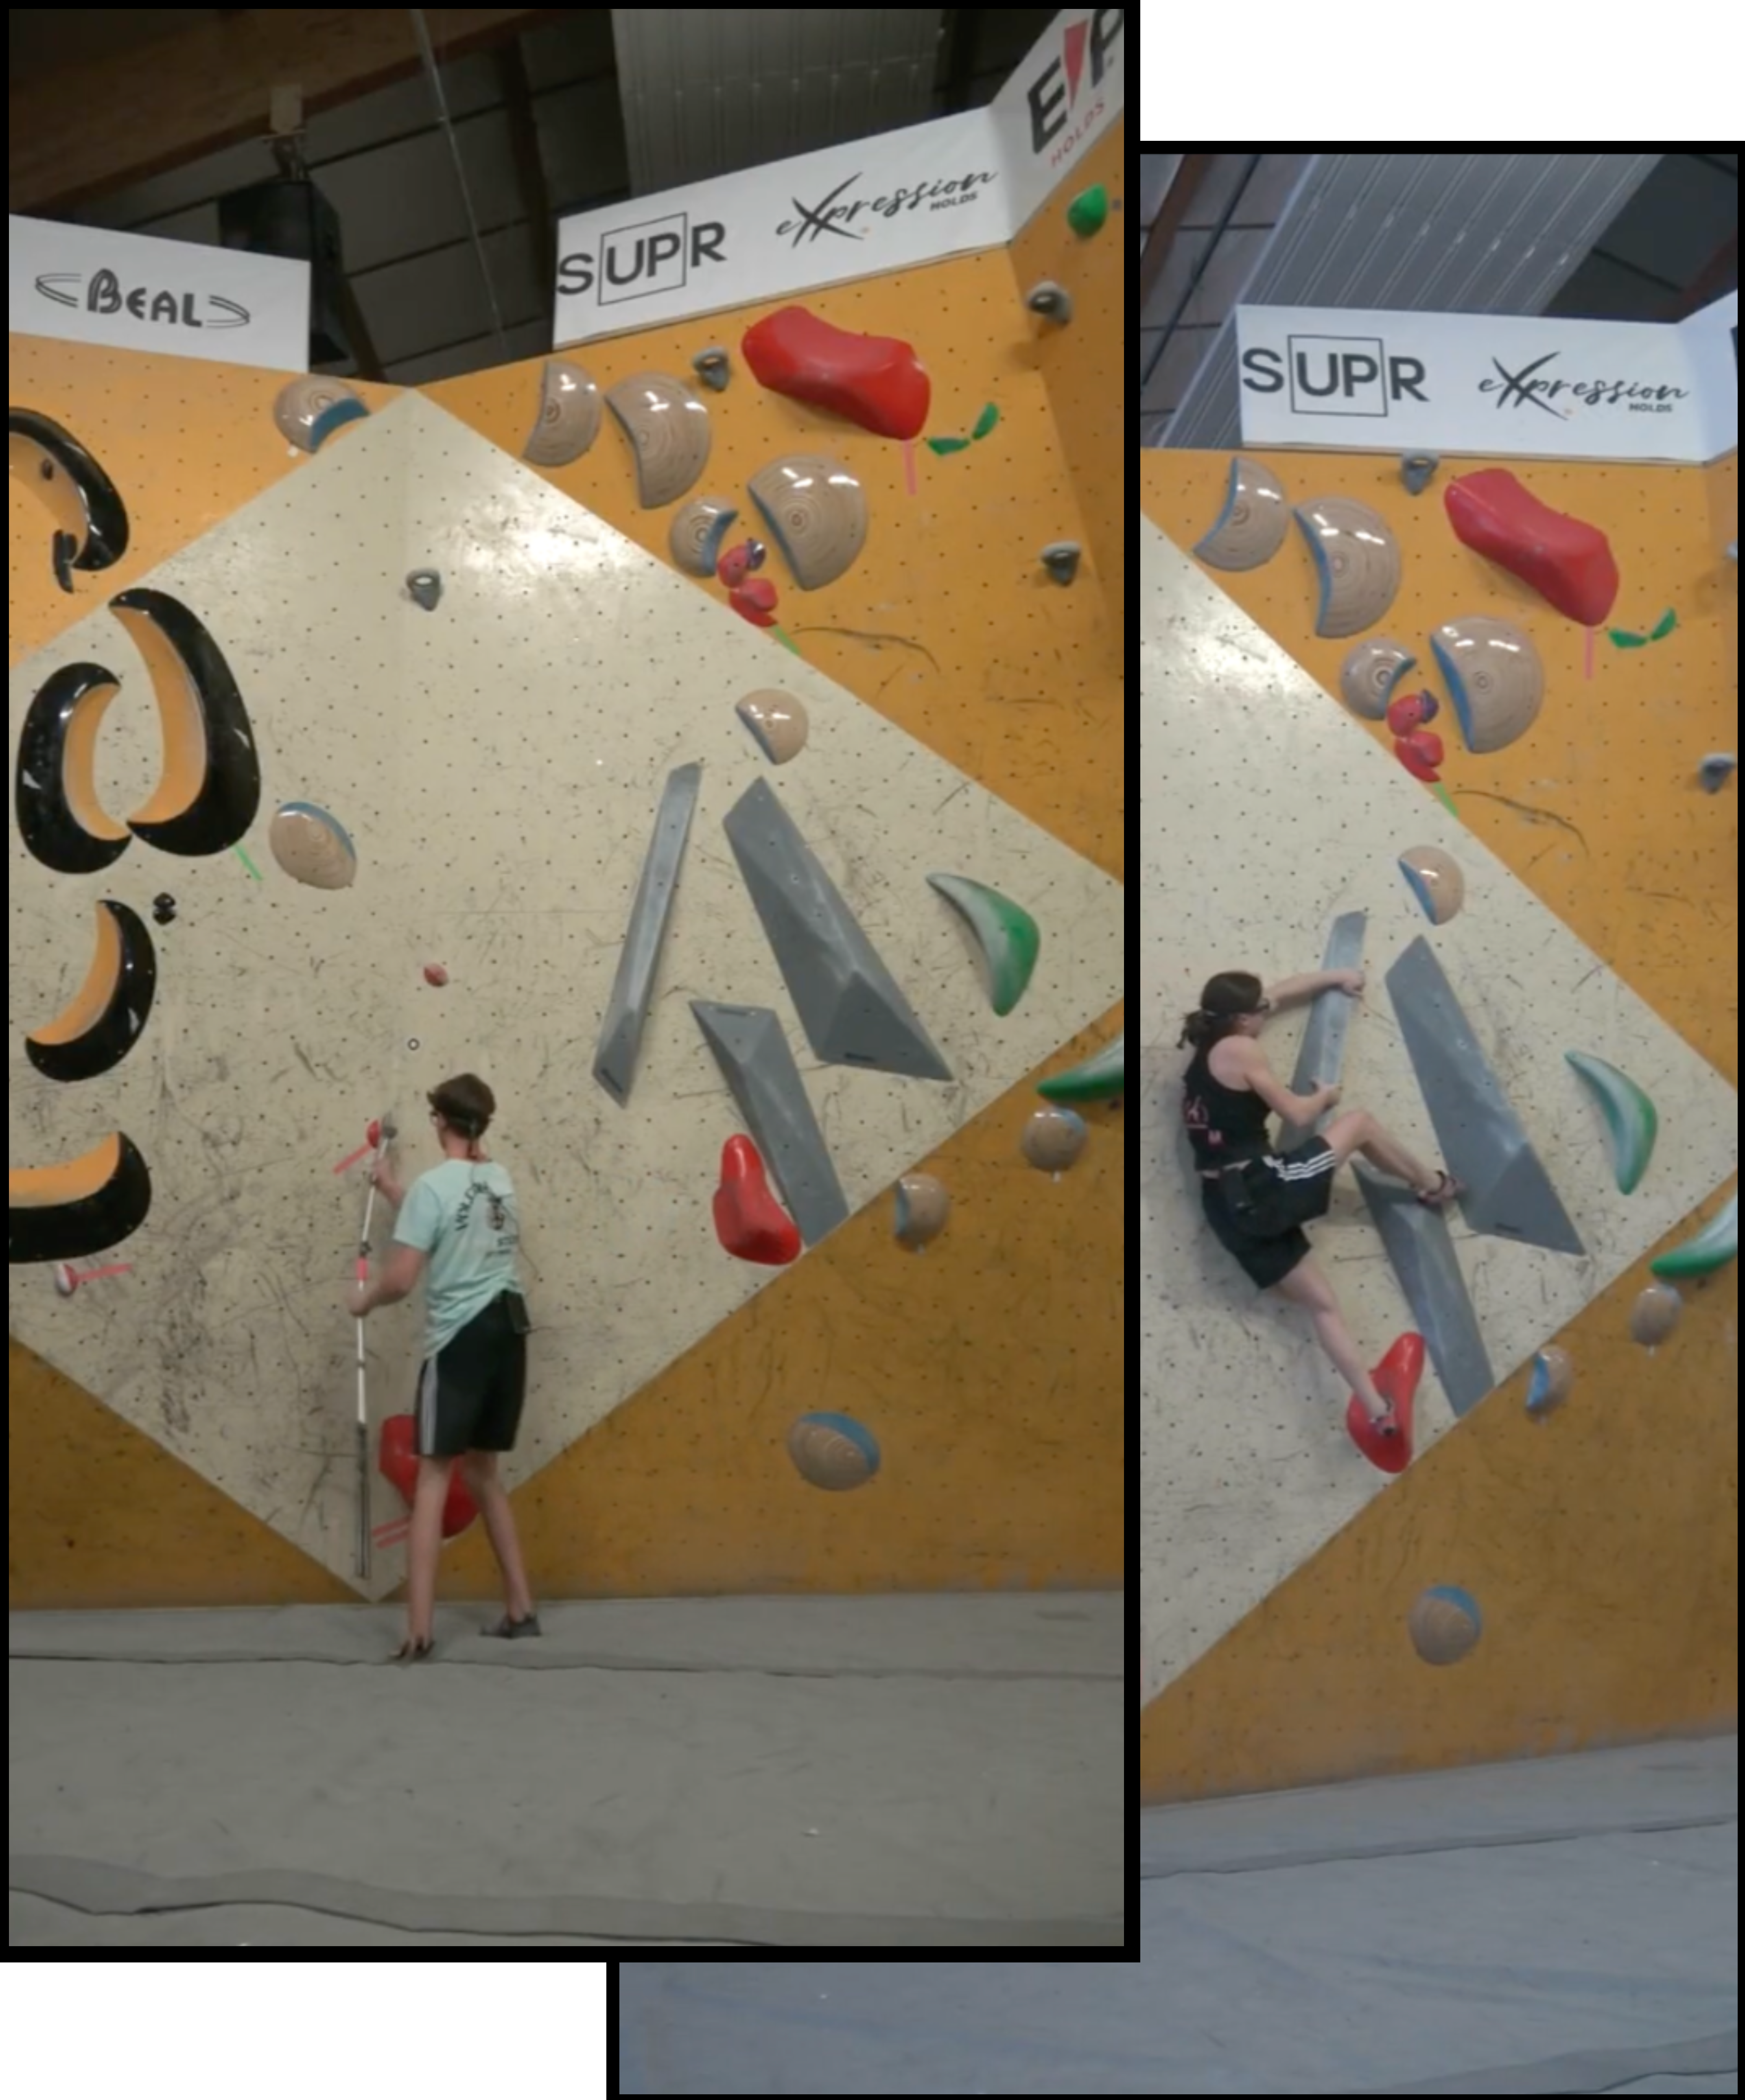
\includegraphics[width=0.75\textwidth]{assets/visuals/images-grimpe.png}

        % TODO: cite the paper from which i took thi graphic.
    \end{minipage}
\end{frame}

% - Present the big project that the research project is part of. Discuss what the part you are working on contributes to the bigger project, such as analyzing climb parts, etc.
% - Present what the part i am working on serves on the big project. For example:
%       - Compare the different metrics between the different climbers.
%       - Feed the climbing parts to a climbing analyzer Model.
%       - Etc.
% - Tell that the project is a Data Science project from start to finish where i need to handle the data pre processing, annotations, models testing, research, etc

% TODO: add another frame for presenting the kind of problem and how it is called Video Action "Segmentation" and make the distinction between the two.